\documentclass[a4paper,french,bookmarks]{book}

\usepackage{./Structure/4PE18TEXTB}
\usepackage{pdfpages}

\newboxans
\renewcommand{\questionsdecours}{\section*{\centering\EBGaramond\Large Questions~ de~ cours}}
\renewcommand{\thechapter}{\arabic{chapter}}
%\renewcommand{\thesection}{\hspace{-11pt}}
%\renewcommand{\thesubsection}{}

\begin{document}
    
    %==============================
    % METADONNEES
    %==============================
    
    \title{Livre des Khôlles de Mathématiques en MP2I (2021-2022)}
    \author{SIAHAAN--GENSOLLEN Rémy}
    \date{\today}
    \hypersetup{
        pdftitle={Livre des Khôlles de Mathématiques en MP2I (2021-2022)},
        pdfauthor={SIAHAAN--GENSOLLEN Rémy},
        pdflang={fr-FR},
        pdfsubject={MP2I, Khôlles},
        pdfkeywords={MP2I, Khôlles, Programmes de Khôlles, 2021-2022}
        pdfstartview=
    }
    
    %==============================
    % MISE EN PAGE
    %==============================
    
    \def\khdate{}
    \titleformat{\chapter}[display]{\normalfont\huge\bfseries}{}{0pt}{
        \begin{tcolorbox}[
            enhanced,
            frame hidden,
            sharp corners,
            spread sidewards    = 5pt,
            halign              = center,
            valign              = center,
            interior style      = {color=main1!20},
            arc                 = 0 cm,
            fontupper           = \color{black}\sffamily\bfseries\huge,
            fonttitle           = \normalfont\color{white}\sffamily\small,
            top                 = 1cm, 
            bottom              = 0.7cm,
            title               = Khôlle \thechapter\ -\ \khdate,
            attach boxed title to bottom center = {
                yshift=\tcboxedtitleheight/2,
            },
            boxed title style = {
                frame code={
                \path[left color=main2!95!gray!90,right color=main1!95!gray!90] 
                    ([xshift=-10mm]frame.north west) -- 
                    ([xshift=10mm]frame.north east) -- 
                    ([xshift=10mm]frame.south east) -- 
                    ([xshift=-10mm]frame.south west) -- 
                    cycle;
                },
                interior engine=empty,
                tikz={rotate=1.5,transform shape}
            }
        ]
            #1
        \end{tcolorbox}%
    }
    \titlespacing*{\chapter}{0pt}{-115pt}{-15pt}
    \titleformat{name=\chapter,numberless}[display]{\normalfont\huge\bfseries}{}{0pt}{
        \begin{tcolorbox}[
            enhanced,
            frame hidden,
            sharp corners,
            spread sidewards    = 5pt,
            halign              = center,
            valign              = center,
            interior style      = {color=main1!20},
            arc                 = 0 cm,
            outer arc           = 0pt,
            leftrule            = 0pt,
            rightrule           = 0pt,
            fontupper           = \color{black}\sffamily\bfseries\huge,
            enlarge left by     = -1in-\hoffset-\oddsidemargin, 
            enlarge right by    = -\paperwidth+1in+\hoffset+\oddsidemargin+\textwidth,
            width               = \paperwidth, 
            left                = 1in+\hoffset+\oddsidemargin, 
            right               = \paperwidth-1in-\hoffset-\oddsidemargin-\textwidth,
            top                 = 1cm, 
            bottom              = 1cm
        ]
            #1
        \end{tcolorbox}%
    }
    \titlespacing*{name=\chapter,numberless}{0pt}{-115pt}{0pt}
    
    %==============================
    % PREMIERE DE COUVERTURE
    %==============================

    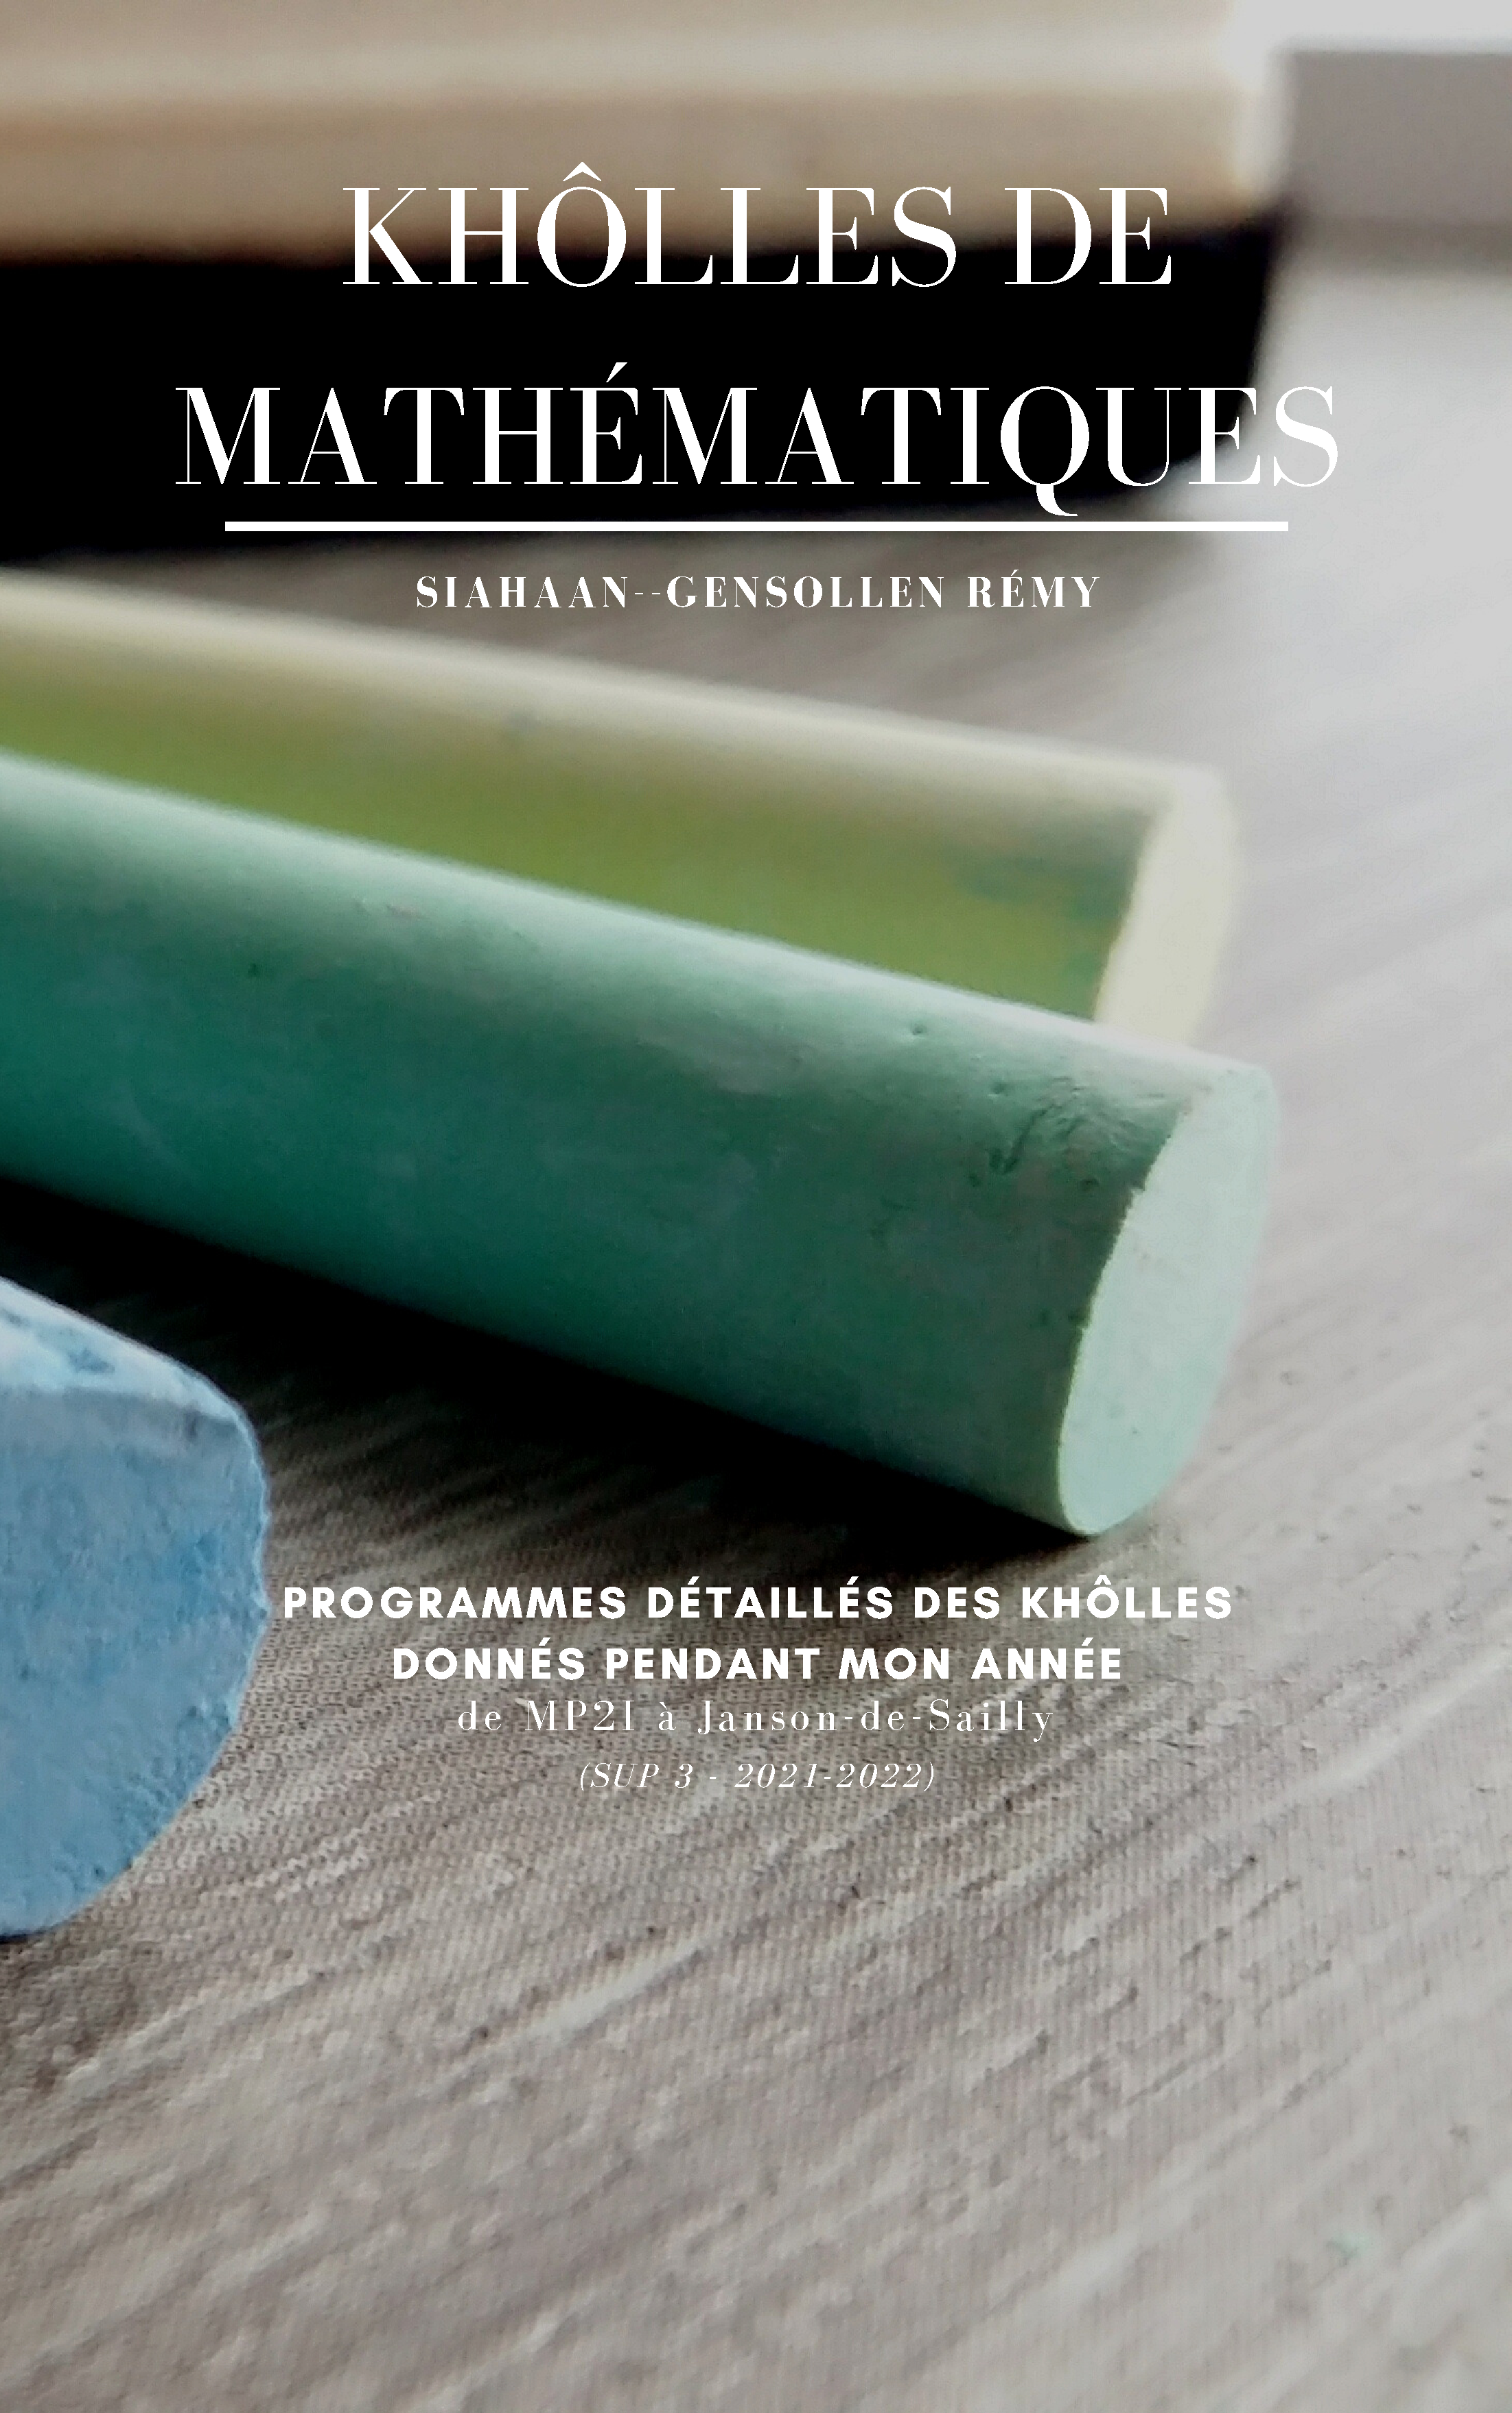
\includepdf[pages={1},scale=1.15,offset=0mm -18mm]{LDCCover.pdf}
    
    %==============================
    % PAGE VIDE
    %==============================
    
    \pagestyle{empty}
    
    %==============================
    % PAGE DE COUVERTURE INTERNE
    %==============================
    
    \begin{titlepage}
	    \begin{center}
	        {\scshape SIAHAAN--GENSOLLEN Rémy \par}
	        \vspace{2cm}
	        {\huge\sffamily Programmes détaillés des\par}
	        \vspace{0.5cm}
	        {\Huge\bfseries\sffamily KHÔLLES DE MATHÉMATIQUES\par}
	        \vspace{1cm}
	        {\Large\textit{donnés pendant mon année de MP2I à
	        Janson-de-Sailly}\\[5pt]\texttt{(SUP 3 - 2021-2022)}\par}
	        \vfill
	        {\large\EBGaramond Dernière compilation le \today\par}
        \end{center}
    \end{titlepage}
    
    %==============================
    % PAGE VIDE
    %==============================
    
    \pagestyle{empty}\text{}\newpage
    
    %==============================
    % STYLE DES EN-TÊTES ET PIEDS DE PAGES
    %==============================
    
    \renewcommand\chaptermark[1]{\markboth{#1}{}}
    
    \fancypagestyle{intro}{
        \fancyhf{}
        \renewcommand{\headrulewidth}{0pt}
        \renewcommand{\footrulewidth}{0pt}\fancyfoot[RO,LE]{\GillSansMTMedium\color{white5}\thepage\;/\;\pageref{LastPage}}
        \fancyhead[CE]{\GillSansMTMedium\color{white5}\bfseries PROGRAMMES DÉTAILLÉS DES KHÔLLES DE MATHÉMATIQUES}
        \fancyhead[CO]{\GillSansMTMedium\color{white5}\text{}}
        \fancyfoot[RE]{\GillSansMTMedium\color{white5}\textbf{MP2I} 2021-2022 \quad Janson-De-Sailly}
        \fancyfoot[LO]{\GillSansMTMedium\color{white5}\text{Préface}} %TAble des matières
    }
    
    \fancypagestyle{toc}{
        \fancyhf{}
        \renewcommand{\headrulewidth}{0pt}
        \renewcommand{\footrulewidth}{0pt}\fancyfoot[RO,LE]{\GillSansMTMedium\color{white5}\thepage\;/\;\pageref{LastPage}}
        \fancyhead[CE]{\GillSansMTMedium\color{white5}\bfseries PROGRAMMES DÉTAILLÉS DES KHÔLLES DE MATHÉMATIQUES}
        \fancyhead[CO]{\GillSansMTMedium\color{white5}\text{}}
        \fancyfoot[RE]{\GillSansMTMedium\color{white5}\textbf{MP2I} 2021-2022 \quad Janson-De-Sailly}
        \fancyfoot[LO]{\GillSansMTMedium\color{white5}\text{Table des matières}} %TAble des matières
    }
    
    \fancypagestyle{plain}{
        \fancyhf{}
        \renewcommand{\headrulewidth}{0pt}
        \renewcommand{\footrulewidth}{0pt}\fancyfoot[RO,LE]{\GillSansMTMedium\color{white5}\thepage\;/\;\pageref{LastPage}}
        \fancyhead[CE]{\GillSansMTMedium\color{white5}\bfseries PROGRAMMES DÉTAILLÉS DES KHÔLLES DE MATHÉMATIQUES}
        \fancyhead[CO]{\GillSansMTMedium\color{white5}\bfseries\leftmark}
        \fancyfoot[RE]{\GillSansMTMedium\color{white5}\textbf{MP2I} 2021-2022 \quad Janson-De-Sailly}
        \fancyfoot[LO]{\GillSansMTMedium\color{white5}Khôlle \thechapter\ \khdate}
    }
    
    %==============================
    % PREFACE 
    %==============================
    
    \chapter*{Préface}
    \thispagestyle{intro}
    \addcontentsline{toc}{chapter}{Préface}
    
    Lorem Ipsum dolor sit amet blablabla.
    
    \pagestyle{intro}
    
    %==============================
    % TABLE DES MATIERES
    %==============================
    
    \newpage
    \tableofcontents\thispagestyle{toc}
    
    
    %==============================
    % Khôlles
    %==============================
    
    \pagestyle{plain}
    
    \setcounter{chapter}{-1}
    
    \def\khdate{intégration des SUP}
    \chapter{Révisions de Tle}
    
    \section*{Ensembles, combinatoire et dénombrement}
    
    \begin{enumerate}
        \ithand Raisonnement par récurrence. Récurrence double, forte.
        
        \ithand Nombre d'éléments d'une réunion d'ensembles, nombre d'éléments d'un produit cartésien. Nombre de $k$-uplets (ou $k$-listes) d'un ensemble à $n$ éléments.
        
        \ithand Définition de $n!$. Notion de permutation, arrangements ($k$-uplets d'éléments distincts d'un ensemble à $n$ éléments), combinaisons. Coefficient binomiaux et propriétés. Relation et triangle de \textsc{Pascal}.
    \end{enumerate}
    
    \section*{Limites de suites et de fonctions}
    
    \begin{enumerate}
        \ithand Limite infinie une suite $(u_n)$ tend vers $+\infty$ si tout intervalle de la forme $[a ; +\infty[$ contient toutes les valeurs $u_n$ à partir d'un certain rang. Suite tendant vers $-\infty$.
        
        \ithand Limite finie d'une suite : la suite $(u_n)$ converge vers le nombre réel $\ell$ si tout intervalle ouvert contenant $\ell$ contient toutes les valeurs $u_n$ à partir d'un certain rang.
        
        \ithand Théorèmes de comparaison, théorème des gendarmes et de convergence monotone (toute suite croissante majorée et décroissante minorée converge). Opérations sur les limites.
        
        \ithand Limite finie ou infinie d'une fonction, en $+\infty$, en $-\infty$, en un point. Théorèmes.
        
        \ithand Limites des fonctions de références étudiées en classe de première : puissances entières $x \mapsto x^n$, racine carrée $x \mapsto \sqrt{x}$, fonction exponentielle $x \mapsto e^x$.
        
        \ithand Croissance comparée de $x \mapsto e^x$ et $x \mapsto x^n$ en $+\infty$.
    \end{enumerate}
    
    \section*{Fonctions usuelles et dérivation}
    
    \begin{enumerate}
        \ithand Fonction logarithme népérien $\ln$, comme réciproque de la fonction exponentielle. Propriétés algébriques, dérivée, variations. Limite en $0$ et en $+\infty$, croissance comparée.
        
        \ithand Fonctions trigonométrique sinus et cosinus. Dérivées, variations, courbes représentatives.
        
        \ithand Composée de deux fonctions et dérivée.
        
        \ithand Dérivée seconde d'une fonction.
        
        \ithand Notion de convexité : définition par la position relative de la courbe représentative et des sécantes. Propriétés. Notion de point d'inflexion.
    \end{enumerate}
    
    \section*{Continuité, primitives, équations différentielles et calcul intégral}
    
    \begin{enumerate}
        \ithand Fonction continue en un point (définition par les limites), sur un intervalle. Toute fonction dérivable est continue. Théorème des valeurs intermédiaires.
        
        \ithand Equation différentielle $y' = f$. Notion de primitive d'une fonction continue sur un intervalle. Primitives des fonctions de référence. Equation différentielle $y' = ay + b$, où $a$ et $b$ sont des nombres réels.
        
        \ithand Définition de l'intégrale d'une fonction continue positive sur un segment $[a; b]$, comme aire sous la courbe représentative de $f$. Notation $\displaystyle\int_a^b f(t)\dif t$.
        
        \ithand Si $f$ est une fonction continue positive sur $[a, b]$, alors la fonction $F_a$ définie sur $[a; b]$ par $F_a(x) = \displaystyle \int_a^x f(t)\textrm{d}t$ est la primitive de $f$ qui s'annule en $a$.
        
        \ithand Relation $F(b) - F(a) = \displaystyle\int_a^b f(x)\textrm{d}x$ où $F$ est une primitive de $f$.
        
        \ithand Propriétés de l'intégrale. Linéarité, positivité et intégration des inégalités. Relation de \textsc{Chasles}.
        
        \ithand Valeur moyenne d'une fonction. Intégration par parties.
    \end{enumerate}
    
    \questionsdecours
    
    \begin{enumerate}
        \item Montrer par récurrence que pour tout entier naturel $n$ non nul, \qquad $1^3 + 2^3 + \dots + n^3 = \left(\displaystyle\frac{n(n+1)}{2}\right)^2$.
        
        \boxans{
            On possède par récurrence simple, selon le prédicat :
            %
            \[ \forall n \in \bdN^*,\qquad H\p{n} : \qquad 1^3 + 2^3 + \dots + n^3 = \sum_{k=1}^n k^3 = \left(\displaystyle\frac{n(n+1)}{2}\right)^2\]
            %
            \begin{enumerate}
                \itt \underline{Initialisation :} On a $1^3 = 1$ et $\p{\dfrac{1(1+1)}{2}}^2 = \p{\dfrac{2}{2}}^2 = 1^2 = 1$ donc $H(1)$ est vrai.
                
                \itt \underline{Hérédité : } Soit $n \in \bdN^*$ tel que $H(n)$ est vrai. On a :
                %
                \begin{align*}
                     1^3 + 2^3 + \dots + n^3 + \p{n+1}^3 &= \dfrac{n^2(n+1)^2}{4} + \p{n+1}^3 = \p{n+1}^2\p{\dfrac{n^2}{4} + (n+1)}\\
                     &=  \dfrac{\p{n+1}^2}{4}\p{n^2 + 4n + 4} = \dfrac{(n+1)^2(n+2)^2}{2^2} = \p{\dfrac{(n+1)(n+2)}{2}}^2
                \end{align*}
                %
                Ainsi $H(n+1)$ est vrai.
                
                \itt \underline{Conclusion :} $H(1)$ est vrai et pour tout entier $n$ nul nul, $H(n) \implies H(n+1)$, donc par principe de récurrence, $1^3 + 2^3 + \dots + n^3 = \left(\displaystyle\frac{n(n+1)}{2}\right)^2$.
            \end{enumerate}
        }
        
        \item Déterminer la limite en $+\infty$ et en $-1$ de la fonction $f$ définie sur $] -1; +\infty [$ par \qquad $f(x) = \displaystyle\frac{4x + 5}{x + 1}$.
        
        \boxans{
            On a $\lim\limits_{x \to -1} x + 1 = 0$ et $\lim\limits_{x \to -1} 4x + 5 = -1$ donc par quotient $\lim\limits_{x \to -1} f(x) = -\infty$.
            
            Par ailleurs $\lim\limits_{x \to +\infty} \dfrac{4x + 5}{x + 1} = \lim\limits_{x \to +\infty} \dfrac{4 + \frac{5}{x}}{1 + \frac{1}{x}} = 4$  donc $\lim\limits_{x \to +\infty} f(x) = 4$.
        }
        
        \item $f$ est la fonction définie sur $[0; 1]$ par \qquad $f(x) = 2 + 3e^{-x}$.
        
        Démontrer qu'il existe au moins un réel $c$ compris entre $0$ et $1$ et tel que $f(c) = 4$.
        
        \boxans{
            La fonction exponentielle est continue sur  $[0; 1]$ donc par quotient la fonction $x \mapsto \dfrac{1}{e^x}$ est continue sur  $[0; 1]$. Par produit puis somme, $f$ est continue sur $[0; 1]$.
            
            On a $f(0) = 2 + 3e^{-0} = 2 + 3 = 5$ et $f(1) = 2 + 3e^{-1} = 2 + \dfrac{3}{e}$. Or $e > 2$ donc $f(1) < 2 + \dfrac{3}{2} = 3,5$.
            
            Ainsi $f(0) > 4 > f(1)$ donc par théorème des valeurs intermédiaires, il existe au moins un réel $c$ compris entre $0$ et $1$ tel que $f(c) = 4$.
        }
        
        \item Déterminer la solution $g$ de l'équation différentielle $y' = y + 1$ telle que $g(1) = 2$.
        
        \boxans{
            Soit $x \in \bdR$. On cherche d'abord la solution constante sous la forme $f(x) = c$, \ie $c + 1 = 0$ donc $c = -1$.
            
            Par ailleurs, $g$ est solution de $y' = y + 1$ si et seulement si $g'(x) = g(x) + 1$, donc $g'(x) = g(x) - f(x)$. Or $f'(x) = 0$ donc $g' = g' - f' = (g - f)'$ donc $g - f$ est solution de l'équation différentielle $y' = y$.
            
            Ainsi, $g(x) - f(x) = g(x) - c = ke^x$ donc $g(x) = ke^x + c = ke^x - 1$.
            
            Enfin, $g(1) = 2$ donc $ke^1 - 1 = 2$ soit $ke = 3$ soit $k = \dfrac{3}{e}$. Donc $g(x) = 3e^{x - 1} -1$.
        }
        
        \item Déterminer, à l'aide de l'intégration par partie, une primitive de $\ln$.
        
        \boxans{
            Soit $x \in \bdRp$, on cherche par exemple à intégrer $\ln t$ pour $t$ entre $1$ et $x$, \ie à calculer $\displaystyle\int_1^t \ln{t}\dif t$.
            
            On intègre par parties, selon $u(t) = t$ (donc $u'(t) = 1$) et $v(t) = \ln t$ (donc $v'(t) = \sfrac{1}{t}$). On a alors :
            %
            \[ \int_1^x \ln{t}\dif t = \int_1^x u'(t)v(t)\dif t = \left[u(t)v(t)\right]_1^x - \int_1^x u(t)v'(t)\dif t = \left[t\ln t\right]_1^x - \int_1^x \dfrac{t}{t}\dif t = x\ln x - \left[t\right]_1^x = x\ln x - x + 1\]
            %
            Une primitive de $x \mapsto \ln x$ est donc $x \mapsto x \ln x - x$.
        }
    \end{enumerate}
    
    \cleardoublepage
    \def\khdate{du 20 au 24 septembre 2021}
    \chapter{Fondements logiques et calculs algébriques}

    \section*{Fondements logiques}
    
    \begin{enumerate}
        \ithand Assertions, connecteurs logiques.
        
        \ithand Implication, réciproque, contraposée, équivalence. Condition
        nécessaire, suffisante.
        
        \ithand Quantificateurs.
        
        \ithand Modes de raisonnement : par disjonction de cas, par l'absurde, par
        contraposée, par analyse-synthèse, par récurrence (simple, double, forte).
    \end{enumerate}
    
    \section*{Calculs algébriques}
    
    \begin{enumerate}
        \ithand Somme et produit d'une famille finie de nombres complexes.
        
        \ithand Propriétés, changements d'indice.
        
        \ithand Sommes et produits télescopiques.
        
        \ithand Sommes usuelles $\displaystyle\sum k$, $\displaystyle\sum k^2$,
        $\displaystyle\sum k^3$, $\displaystyle\sum x^k$, suites arithmétiques,
        géométriques.
        
        \ithand Factorisation de $a^n - b^n$.
        
        \ithand Sommes doubles. Produit de deux sommes finies, sommes triangulaires.
        
        \ithand Factorielle. Coefficients binomiaux. Symétrie.
        
        \ithand Triangle de \textsc{Pascal}. Formule du chef  $\dbinom{n}{k} =
        \dfrac{n}{k}\dbinom{n-1}{k-1}$. Binôme de \textsc{Newton} dans $\bdR$.
    \end{enumerate}
    
    \questionsdecours
    
    \begin{enumerate}
        \item Montrer que $\sqrt{2}$ est irrationnel.
        
        \boxans{
            On raisonne par l'absurde. Pour cela, on suppose que $\sqrt{2} \in \bdQ$. Ainsi, $\sqrt{2}$ peut s'écrire sous la forme d'une quotient de deux entiers premiers entre eux (tous deux strictement positifs puisque $\sqrt{2} > 0$), \ie :
            %
            \[ \exists \p{p, q} \in \p{\bdN^*}^2,\qquad \sqrt{2} = \dfrac{p}{q} \qquad\et\qquad \pgcd\p{p, q} = 1 \]
            %
            Au carré, on obtient donc $2 = \dfrac{p^2}{q^2}$, soit $2q^2 = p^2$. Ainsi, $p^2$ est divisible par $2$. Or :
            %
            \[ \forall k \in \bdZ,\qquad k \equiv 1 \ \intc{2} \implies k^2 \equiv 1 \intc{2} \qquad\text{donc par contraposée} \qquad k^2 \equiv 0 \ \intc{2} \implies k \equiv 0 \intc{2} \]
            %
            Ainsi, $p$ est aussi divisible par $2$, ce qui livre l'existence d'un $p' \in \bdN^*$ tel que $p = 2p'$
            %
            \[ 2q^2 = p^2 \qquad\text{donc}\qquad 2q^2 = \p{2p'}^2 \qquad\text{donc}\qquad 2q^2 = 4p'^2 \qquad\text{donc}\qquad q^2 = 2p'^2\]
            %
            Ainsi $q^2$ est divisible par $2$, et donc que $q$ l'est aussi. On remarque alors que $p$ et $q$ partagent $2$ en facteur commun, ils ne peuvent donc être premiers entre eux $\p{\pgcd\p{p, q} \geq 2}$. C'est une contradiction avec l'hypothèse énoncée plus haut. Par l'absurde, on en déduit donc que $\sqrt{2} \not\in \bdQ$.
        }
        
        \item Montrer qu'il existe un unique couple $\p{f, g}$ de fonctions de $\bdR$ dans $\bdR$ avec $f$ paire, $g$ impaire et telles que $\forall x \in \bdR$,\qquad $e^x = f\p{x} + g\p{x}$.
        
        \boxans{
            On procède par analyse-synthèse. \underline{Analyse :} soient $\p{f, g} \in \bcF\p{\bdR,\bdR}^2$ deux fonctions telles que $\exp = f + g$. Soit $x \in \bdR$ : si $f$ est paire et $g$ est impaire, alors $f(-x) = f(x)$ et $g(-x) = -g(x)$ donc $e^{-x} = f(-x) + g(-x) = f(x) - g(x)$. On a donc le système $\left\lbrace\begin{array}{cc}
                e^x &= f(x) + g(x)  \\
                e^{-x} &= f(x) - g(x) 
            \end{array}\right.$, donc $\left\lbrace\begin{array}{cc}
                f(x) &= \dfrac{e^x + e^{-x}}{2}  \\
                g(x) &= \dfrac{e^x - e^{-x}}{2}
            \end{array}\right.$.
            
            \underline{Synthèse :} On vérifie facilement que $\dfrac{e^x + e^{-x}}{2} + \dfrac{e^x - e^{-x}}{2} = e^x$ donc il existe bien un unique couple $\p{f, g}$ de fonctions de $\bdR$ dans $\bdR$ avec $f$ paire et $g$ impaire et telles que $\exp = f + g$.
        }
        
    \item Montrer qu'il n'existe pas de suite d'entiers naturels infinie strictement décroissante.
    
    \noafter
    %
    \boxans{
        \begin{property*}{Majoration d'une suite d'entiers strictement décroissante}{}
            Soit \hg{$\suite{u_n} \in \bdZ^\bdN$} une suite d'\hg{entiers relatifs strictement décroissante}. On a
            %
            \[ \hg{\forall n \in \bdN,\qquad u_n \leq u_0 - n}\]
            %
        \end{property*}
    }
    %
    \nobefore
    %
    \begin{nproof}
         Soit $\suite{u_n} \in \bdZ^\bdN$ une suite d'entiers relatifs strictement décroissante. On montre par récurrence le prédicat :
        %
        \[ \forall n \in \bdN,\qquad H(n) : u_n \leq u_0 - n \]
        %
        \begin{enumerate}
            \itt \underline{Initialisation :} $u_0 = u_0 \leq u_0 - 0$ donc $H(0)$ est vrai.
            
            \itt \underline{Hérédité :} Soit $n \in \bdN$ tel que $H(n)$ est vrai. La suite $\suite{u_n}$ est strictement décroissante donc $u_{n+1} < u_n$. Or $u_{n+1} \in \bdZ$ et $u_n \in \bdZ$ donc $u_{n+1} \leq u_n - 1$. Par HR, $u_{n+1} \leq u_0 - (n+1)$, donc $H(n+1)$ est vrai.
            
            \itt \underline{Conclusion :} $H(0)$ est vrai et pour tout $n \in \bdN$, on a $H(n) \implies H(n+1)$ donc pour tout entier naturel non nul $n \in \bdN^*$, on a $\forall n \in \bdN,\qquad u_n \leq u_0 - (n+1)$.
        \end{enumerate}
    \end{nproof}
    %
    \yesafter
    %
    \boxans{
        Supposons maintenant par l'absurde qu'il existe une suite $\suite{v_n} \in \bdN^\bdN$ d'entiers naturels infinie strictement décroissante.
        %
        \begin{enumerate}
            \itt D'une part, puisque la suite est infinie et que c'est une suite d'entiers naturels, alors $v_{v_0 + 1}$ existe et $v_{v_0 + 1} \geq 0$.
            
            \itt D'autre part, puisque $\bdN \subset \bdZ$, la suite $\suite{v_n}$ vérifie la propriété précédente, et ainsi $v_{v_0 + 1} \leq v_0 - (v_0 + 1)$ donc $v_{v_0 + 1} \leq -1$.
        \end{enumerate}
        %
        Ainsi $0 \leq v_{v_0 + 1} \leq -1$ soit $0 \leq -1$, ce qui est absurde. Il n'existe donc pas de suite d'entiers naturels infinie strictement décroissante.
         
    }
    %
    \yesbefore
    
    \item Montrer que $\displaystyle\sum_{k = 1}^n k^2 = \dfrac{n(n+1)(2n + 1)}{6}$.
    
    \noafter
    %
    \boxans{
        \begin{property*}{Somme des carrés}{}
            Soit un entier naturel non nul \hg{$n \in \bdN^*$}. On a :
            %
            \[ \hg{\forall n \in \bdN^*,\qquad 1^2 + 2^2 + \dots + n^2 = \displaystyle\sum_{k = 1}^n k^2 = \dfrac{n(n+1)(2n + 1)}{6} } \]
        \end{property*}
    }
    %
    \nobefore
    \yesafter
    %
    \begin{nproof}
        On possède par récurrence simple, selon le prédicat :
        %
            \[ \forall n \in \bdN^*,\qquad H\p{n} : \qquad 1^2 + 2^2 + \dots + n^2 = \displaystyle\sum_{k = 1}^n k^2 = \dfrac{n(n+1)(2n + 1)}{6}\]
            %
            \begin{enumerate}
                \itt \underline{Initialisation :} On a $1^2 = 2$ et $\dfrac{1\p{1 + 1}\p{2\times 1 + 1}}{6} = \dfrac{1\times2\times3}{6} = \dfrac{6}{6} = 1$ donc $H(1)$ est vrai.
                
                \itt \underline{Hérédité : } Soit $n \in \bdN^*$ tel que $H(n)$ est vrai. On a :
                %
                \begin{align*}
                     \sum_{k=1}^{n+1} k^2 = \sum_{k=1}^n k^2 + (n+1)^2 = \dfrac{n(n+1)(2n+1)}{6} + (n+1)^2 = \dfrac{n+1}{6}\p{2n^2 + 7n + 6}
                \end{align*}
                %
                Or $(n+2)(2n+3) = 2n^2 + 7n + 6$ donc $\displaystyle \sum_{k=1}^{n+1} k^2 = \dfrac{(n+1)(n+2)(2n+3)}{6}$, ainsi $H(n+1)$ est vrai.
                
                \itt \underline{Conclusion :} $H(1)$ est vrai et pour tout entier $n$ nul nul, $H(n) \implies H(n+1)$, donc par principe de récurrence, pour tout entier naturel non nul $n \in \bdN^*$, on a $\displaystyle\sum_{k = 1}^n k^2 = \dfrac{n(n+1)(2n + 1)}{6}$.
            \end{enumerate}
    \end{nproof}
    %
    \yesbefore
    
    \item Calcul de $\displaystyle \sum_{1 \leq i, j \leq n} \min{i, j}$.
    
    \boxans{
        \begin{align*}
            \sum_{1 \leq i, j \leq n} \min{i, j} &= \sum_{i = 1}^n \sum_{j = 1}^n \min{i, j} =  \sum_{i = 1}^n  \left(\sum_{j=1}^i \min{i, j} + \sum_{j=i+1}^n \min{i, j}\right) = \sum_{i = 1}^n \left(\sum_{j=1}^i j + \sum_{j=1+1}^n i\right)\\
            &= \sum_{i=1}^n \p{\dfrac{i(i+1)}{2} + (n-i)i} = \sum_{i=1}^n \p{\dfrac{i^2}{2} + \dfrac{i}{2} + ni - i^2} = \p{\dfrac{1}{2} + n}\sum_{i=1}^n -\dfrac{1}{2}\sum_{i=1}^n i^2\\
            &= \p{\dfrac{1}{2} + n}\dfrac{n(n+1)}{2} -\dfrac{1}{2}\dfrac{n(n+1)(2n+3)}{6} = \dfrac{n}{2}\p{\dfrac{3(n+1)}{6} + \dfrac{6n(n+1)}{6} + \dfrac{(n+1)(2n+1)}{6}}\\
            &= \dfrac{n(n+1)}{12}\p{3 + 6n + 2n + 1} = \dfrac{n(n+1)(4 + 8n)}{12} = \dfrac{n(n+1)(2n+1)}{3}
        \end{align*}
    }
    
    \item Calculer $\displaystyle\sum_{k=1}^n k2^k$ en utilisant $k = \displaystyle\sum_{i=1}^k 1$.
    
    \boxans{
        \begin{align*}
            \sum_{k=1}^n k2^k &= \sum_{k=1}^n \p{\sum_{i=1}^k 1}2^k = \sum_{k=1}^n\sum_{i=1}^k 2^k = \sum_{1 \leq i \leq k \leq n} 2^k = \sum_{i=1}^n \sum_{k=i}^n 2^k = \sum_{i=1}^n 2^i\dfrac{2^{n-i+1} -1 }{2 - 1} = \sum_{i=1}^n 2^{n+1} - \sum_{i=1}^n 2^i\\
            &= n2^{n+1} - 2\dfrac{2^n - 1}{2 - 1} = n2^{n+1} - 2\p{2^n - 1} = 2^{n+1}(n-1) + 2
        \end{align*}
    }
    
    \item Montrer la formule du binôme de \textsc{Newton}.
    
    \noafter
    %
    \boxans{
        \begin{theorem*}{binôme de Newton}{}
            Soient deux complexes \hg{$\p{a, b} \in \bdC^2$} et un entier \hg{$n \in \bdN$}. On a :
            %
            \[ \hg{ \p{a + b}^n = \sum_{k=0}^n \binom{n}{k} a^kb^{n-k}}\]
        \end{theorem*}
    }
    %
    \nobefore
    \yesafter
    %
    \begin{nproof}
        Soient deux complexes $\p{a, b} \in \bdC^2$. On procède par récurrence simple selon le prédicat :
        %
        \[ \forall n \in \bdN,\qquad H(n) : \p{a + b}^n = \sum_{k=0}^n \binom{n}{k} a^kb^{n-k}\]
        %
        \begin{enumerate}
            \itt \underline{Initialisation :} On a $(a + b)^0 = 0$ et $\sum_{k = 0}^0 \binom{0}{k}a^kb^{0-k} = \binom{0}{0}a^0b^0 = 0$, donc $H(0)$ est vrai.
            
            \itt \underline{Héridité :} Soit $n \in \bdN$ tel que $H(n)$ est vrai. On a :
            %
            \begin{align*}
                (a + b)^{n+1} &= (a+b)(a+b)^n = (a+b)\p{\sum_{k=0}^n \binom{n}{k} a^kb^{n-k}} = \sum_{k=0}^n \binom{n}{k} a^{k+1}b^{n-k} + \sum_{k=0}^n \binom{n}{k} a^kb^{n+1-k}\\
                &= \sum_{k=1}^{n+1} \binom{n}{k - 1} a^kb^{n+1-k} + \sum_{k=0}^n \binom{n}{k} a^kb^{n+1 - k}\\
                &= \sum_{k=1}^n \intc{\binom{n}{k-1} + \binom{n}{k}}a^kb^{n+1-k} + \binom{n}{n}a^{n+1}b^0 + \binom{n}{0}a^0b^{n+1}\\
                &= \sum_{k=1}^n \binom{n+1}{k} a^kb^{n+1-k} + \binom{n+1}{n+1}a^{n+1}b^{0} + \binom{n+1}{0} a^0b^{n+1} = \sum_{k=0}^{n+1} \binom{n+1}{k} a^kb^{n+1-k}
            \end{align*}
            %
            Donc $H(n+1)$ est vrai.
            %
            \itt \underline{Conclusion :} $H(1)$ est vrai et pour tout entier $n$ nul nul, $H(n) \implies H(n+1)$, donc par principe de récurrence, pour tout entier $n \in \bdN$, on a :
            %
            \[ \p{a + b}^n = \sum_{k=0}^n \binom{n}{k} a^kb^{n-k}\]
        \end{enumerate}
    \end{nproof}
    %
    \yesbefore
    
    \end{enumerate}
    
    \cleardoublepage
    \def\khdate{du 27 septembre au 1er octobre 2021}
    \chapter{Ensembles et applications}
    
    \section*{Ensembles}
    
    \begin{enumerate}
        \ithand Inclusion, ensemble vide, égalité.
        
        \ithand Opérations : union, intersection, différence, complémentaire.
        
        \ithand Partie, sous-ensemble, ensemble des parties.
        
        \ithand Produit cartésien.
    \end{enumerate}
    
    \section*{Applications}
    
    \begin{enumerate}
        \ithand Définitions : ensemble de départ, d'arrivée, graphe, image, antécédent, égalité. 
        
        \ithand Application identité, exemples divers. Restriction, prolongement, exemples.
        
        \ithand Injection, surjection, bijection.
        
        \ithand Composée de deux applications.
        
        \ithand Liens entre les composées d'applications et les propriétés de surjectivité, injectivité.
        
        \ithand Bijection réciproque, composée de de bijections et réciproque. Involution.
        
        \ithand Image directe et réciproque d'une partie.
        
        \ithand Images directes et réciproques d'une inclusion, intersection, complémentaire.
        
        \ithand Fonction indicatrice, deux ensembles sont égaux s'ils ont même fonction indicatrice.
    \end{enumerate}
    
    \questionsdecours
    
    \begin{center}
        \begin{minipage}{0.8\linewidth}
            \begin{tcolorbox}[
                breakable,
                enhanced,
                frame hidden,
                interior style      = {left color=main4!15,right color=main2!12},
                sharp corners       = downhill,
                arc                 = 0 cm,
                boxrule             = 0.5pt,
                drop fuzzy shadow   = black!40!white,
                nobeforeafter,
            ]
                \centering\textbf{\sffamily Note aux colleurs :} On posera à chaque élève une définition et une démonstration.
            \end{tcolorbox}
        \end{minipage}
    \end{center}

    \begin{enumerate}
        \item Définitions de l'inclusion, union, intersection, différence ensembliste et complémentaire.
        
        \noafter
        %
        \boxans{
            %
            \begin{definition*}{Inclusion et partie (sous-ensemble)}{}
                Soient deux ensembles \hg{$A$} et \hg{$B$}. On dit que \hg{$A$ est inclus dans $B$}, que \hg{$A$ est une partie} (ou un \hg{sous-ensemble}) \hg{de $B$} lorsque :
                %
                \[ \hg{\forall x, \qquad x \in A \implies x \in B}\]
            \end{definition*}
            %
        }
        %
        \nobefore
        %
        \begin{notation}
                La proposition \hg{$A$ est inclus dans $B$} se note \hg{$A \subset B$}.
        \end{notation}
        %
        \boxans{
            \begin{definition*}{Union, intersection, différence ensembliste et complémentation}{}
                Soient deux ensembles \hg{$A$} et \hg{$B$}.
                
                \begin{enumerate}
                    \itstar On appelle \hg{intersection de $A$ et $B$} l'ensemble $\hg{\ens{x \enstq x \in A \et x \in B}}$.
                    
                    \itstar On appelle \hg{union de $A$ et $B$} l'ensemble $\hg{\ens{x \enstq x \in A \ou x \in B}}$.
                    
                    \itstar On appelle la différence ensembliste \hg{$A$ privé de $B$} (ou \hg{$A$ moins $B$}) l'ensemble $\hg{\ens{x \enstq x \in A \et x \not\in B}}$.
                    
                    \itstar Si \hg{$A$ est inclus dans $B$}, on appelle \hg{complémentaire de $A$ dans $B$} l'ensemble \hg{$B$ privé de $A$}.
                \end{enumerate}
            \end{definition*}
        }
        %
        \yesafter
        %
        \begin{notation}
            \begin{enumerate}
                \itt L'\hg{intersection de $A$ et $B$} est notée \hg{$A \cap B$}.
                
                \itt L'\hg{union de $A$ et $B$} est notée \hg{$A \cup B$}.
                
                \itt L'ensemble \hg{$A$ privé de $B$} est noté \hg{$A \backslash B$} ou \hg{$A - B$}.
                
                \itt Le \hg{complémentaire de $A$ dans $B$} est noté \hg{$\complement_B A$},\hg{$B \backslash A$}, \hg{$B - A$}, ou, lorsqu'il n'y a pas confusion, \hg{$\overline A$}.
            \end{enumerate}
        \end{notation}
        %
        \yesbefore
        
        \newpage
        
        \item Définition de $\bcP(E)$ et donner $\bcP\p{\ens{a, b, c}}$.
        
        \noafter
        %
        \boxans{
            \begin{definition*}{Ensemble des parties}{}
                Soit un ensemble \hg{$E$}. On appelle \hg{ensemble des parties de $E$} l'ensemble $\hg{\ens{F \enstq F \subset E}}$.
            \end{definition*}
        }
        %
        \nobefore
        %
        \begin{notation}
            L'\hg{ensemble des parties de $E$} est noté \hg{$\bcP(E)$}.
        \end{notation}
        %
        \yesafter
        %
        \boxans{
            On a $\bcP\p{\ens{a, b, c}} = \ens{\emptyset, \ens{a}, \ens{b}, \ens{c}, \ens{a, b}, \ens{a, c}, \ens{b, c}, \ens{a, b, c}}$.
        }
        %
        \yesbefore
        
        \item Définition et caractérisation de l'injectivité, surjectivité.
        
        \noafter
        %
        \boxans{
            \begin{definition*}{Injectivité et  surjectivité}{}
                Soient deux ensembles \hg{$E$ et $F$} et \hg{$f \in \bcF\p{E, F}$} une application de $E$ dans $F$.
                %
                \begin{enumerate}
                    \itstar On dit que \hg{$f$ est injective} lorsque \hg{tout élément de $F$ admet au plus un antécédent par $f$}.
                    
                    \itstar On dit que \hg{$f$ est surjective} lorsque \hg{tout élément de $F$ admet au moins un antécédent par $f$}.
                \end{enumerate}
            \end{definition*}
            %
            \begin{theorem*}{Caractérisation de l'injectivité}{}
                 Soient deux ensembles \hg{$E$} et \hg{$F$} et \hg{$f \in \bcF\p{E, F}$} une application de $E$ dans $F$. On a :
                 %
                 \[ \hg{f \ \text{est injective} \qquad\iff\qquad \forall \p{x, y} \in E^2,\qquad f(x) = f(y) \implies x = y} \]
            \end{theorem*}
        }
        %
        \nobefore
        %
        \begin{nproof}
            Soient deux ensembles $E$ et $F$ et $f \in \bcF\p{E, F}$ une application de $E$ dans $F$.
            %
            \begin{enumerate}
                \itt $\boxed{\implies}$ Soit $\p{x, y} \in E^2$ tel que $f\p{x} = f\p{y}$ et l'image réciproque $E = f^{-1}\p{f(x)} = f^{-1}\p{f(y)}$. On a $x \in E$ et $y \in E$. Si $f$ est injective, alors $\Card{E} \leq 1$ par définition donc $x = y$.
                
                \itt $\boxed{\impliedby}$ Supposons que $\forall (x, y) \in E^2, f(x) = f(y) \implies x = y$. Soit $z \in F$, si $z$ a un antécédent $x$, alors pour tout autre antécédent $y$, on a $f(x) = z = f(y)$ donc $x = y$, donc $z$ a au plus un antécédent.
            \end{enumerate}
            %
            \text{}\\[-20pt]
        \end{nproof}
        %
        \boxans{
            \begin{theorem*}{Caractérisation de la surjectivité}{}
                Soient deux ensembles \hg{$E$} et \hg{$F$} et \hg{$f \in \bcF\p{E, F}$}. Les propositions suivantes sont équivalentes :
                %
                \begin{psse}
                    \item \hg{$f$ est surjective}
                    \item \hg{$\forall y \in F,\qquad \exists x \in E,\qquad f(x) = y$}
                    \item \hg{$f(E) = \Imm(f) = F$}
                \end{psse}
            \end{theorem*}
        }
        %
        \yesafter
        %
        \begin{nproof}
            Soient deux ensembles $E$ et $F$ et $f \in \bcF\p{E, F}$ une application de $E$ dans $F$.
            
            \begin{enumerate}
                \itt $\boxed{\pssenum{i} \iff \pssenum{ii}}$ L'équivalence s'obtient en formalisant la définition.
                
                \itt $\boxed{\pssenum{ii} \implies \pssenum{iii}}$ Supposons que $\forall y \in F, \exists x \in E, f(x) = y$. Soit $y \in F$, il existe $x \in E$ tel que $f(x) = y$ donc $y \in \Imm{f}$, et donc $F \subset \Imm{f}$. Or $\Imm{f} \subset F$ par définition, donc $\Imm{f} = F$.
                
                \itt $\boxed{\pssenum{ii} \impliedby \pssenum{iii}}$ Supposons que $\Imm{f} = F$. Soit $y \in F$, alors $y \in \Imm{f}$ donc $\exists x \in E$ tel que $f\p{x} = y$.
            \end{enumerate}
        \end{nproof}
        %
        \yesbefore
        
        \item Définition de l'image directe et de l'image réciproque d'une partie.
        
        \noafter
        %
        \boxans{
            \begin{definition*}{Image directe et réciproque d'une partie}{}
                Soient deux ensembles \hg{$E$} et \hg{$F$}, deux parties \hg{$E' \subset E$} et\hg{$F' \subset F$}, et une application \hg{$f \in \bcF\p{E, F}$}.
                
                \begin{enumerate}
                    \itstar On appelle \hg{image directe de $E'$ par $f$} l'ensemble $\hg{\ens{y \in F \enstq \exists x \in E',\quad f(x) = y}}$.
                    
                    \itstar On appelle \hg{image réciproque de $F'$ par $f$} l'ensemble $\hg{\ens{x \in E \enstq f(x) \in F'}}$.
                \end{enumerate}
            \end{definition*}
        }
        %
        \nobefore
        \yesafter
        %
        \begin{notation}
            L'\hg{image directe de $E'$ par $f$} se note \hg{$f(E')$}. L'\hg{image réciproque de $F'$ par $f$} se note \hg{$f^{-1}(F')$}.
        \end{notation}
        %
        \yesbefore
        
        \item Montrer que si $f : E \to F$ et $g : F \to G$ sont injectives, alors $g \circ f$ est injective.
        
        \noafter
        %
        \boxans{
            \begin{property*}{Composée d'injections}{}
                Soient trois ensembles \hg{$E$}, \hg{$F$} et \hg{$G$} et deux applications \hg{$f \in \bcF\p{E, F}$} et \hg{$g \in \bcF\p{F, G}$}.
                %
                \[ \hg{f \et g \ \text{sont injectives} \implies g \circ f \ \text{est injective}} \]
            \end{property*}
        }
        %
        \nobefore
        \yesafter
        %
        \begin{nproof}
            Soient trois ensembles $E$, $G$ et $F$ et deux applications $f \in \bcF\p{E, F}$ et $g \in \bcF\p{F, G}$, telles que $f$ et $g$ sont injectives. Soient $\p{x, y} \in G^2$.
            %
            \[ g \circ f \p{x} = g \circ f \p{y} \implies g\p{f\p{x}} = g\p{f\p{y}} \underset{\text{injectivité de } g}{\implies} f\p{x} = f\p{y} \underset{\text{injectivité de } f}{\implies} x = y\]
            %
            Donc par caractérisation, $g \circ f$ est injective.
        \end{nproof}
        %
        \yesbefore
        
        \item Montrer que si $f : E \to F$ et $g : F \to G$ sont surjectives, alors $g \circ f$ est surjective.
        
        \noafter
        %
        \boxans{
            \begin{property*}{Composée d'injections}{}
                Soient trois ensembles \hg{$E$}, \hg{$F$} et \hg{$G$} et deux applications \hg{$f \in \bcF\p{E, F}$} et \hg{$g \in \bcF\p{F, G}$}.
                %
                \[ \hg{f \et g \ \text{sont surjectives} \implies g \circ f \ \text{est surjective}} \]
            \end{property*}
        }
        %
        \nobefore
        \yesafter
        %
        \begin{nproof}
            Soient trois ensembles $E$, $G$ et $F$ et deux applications $f \in \bcF\p{E, F}$ et $g \in \bcF\p{F, G}$, telles que $f$ et $g$ sont surjectives.
            %
            \[ g \circ f\p{E} = g\p{f\p{E}} \eq{\text{surjectivité de } f} g\p{F} \eq{\text{surjectivité de } g} G\]
            %
            Donc par caractérisation, $g \circ f$ est surjective.
        \end{nproof}
        %
        \yesbefore
        
        \item Montrer que si $f : E \to F$ et $g : F \to G$ sont bijectives, alors $g \circ f$ est bijective et exprimer $\p{g \circ f}^{-1}$ en fonction de $f^{-1}$ et $g^{-1}$.
        
        \noafter
        %
        \boxans{
            \begin{property*}{Composée de bijections}{}
                Soient trois ensembles \hg{$E$}, \hg{$F$} et \hg{$G$} et deux applications \hg{$f \in \bcF\p{E, F}$} et \hg{$g \in \bcF\p{F, G}$}.
                %
                \[ \hg{f \et g \ \text{sont bijectives} \implies g \circ f \ \text{est bijective}} \]
            \end{property*}
        }
        %
        \nobefore
        %
        \begin{nproof}
            Soient trois ensembles $E$, $G$ et $F$ et deux applications $f \in \bcF\p{E, F}$ et $g \in \bcF\p{F, G}$, telles que $f$ et $g$ sont bijectives. Alors $f$ et $g$ sont toutes deux injectives, donc $g \circ f$ est injective.
            
            De même, $f$ et $g$ sont toutes deux surjectives, donc $g \circ f$ est surjective.
            
            Puisque $g \circ f$ et injective et surjective, $g \circ f$ est bijective.
        \end{nproof}
        %
        \boxans{
            \begin{property*}{Réciproque d'une composée}{}
                Soient trois ensembles \hg{$E$}, \hg{$F$} et \hg{$G$} et deux applications \bf{bijectives }\hg{$f \in \bcF\p{E, F}$} et \hg{$g \in \bcF\p{F, G}$}.
                
                \[ \hg{ \p{g \circ f}^{-1} = f^{-1} \circ g^{-1}}\]
            \end{property*}
        }
        %
        \begin{nproof}
            Soient trois ensembles $E$, $G$ et $F$ et deux applications $f \in \bcF\p{E, F}$ et $g \in \bcF\p{F, G}$, telles que $f$ et $g$ sont bijectives. Le résultat précédent livre la bijectivité de $g \circ f$. Par associativité de la composée, on a :
            %
            \[ 
                \p{g \circ f} \circ f^{-1} \circ g^{-1} = g \circ \p{f \circ f^{-1}} \circ g^{-1} = g \circ g^{-1} = \id_G
            \]
            De même, on obtient :
            %
            \[
                f^{-1} \circ g^{-1} \circ \p{g \circ f} = f^{-1} \circ \p{g^{-1} \circ g} \circ f = f^{-1} \circ f = \Id_E
            \]
            %
            Par définition, $f^{-1} \circ g^{-1}$ est donc la réciproque de $g \circ f$ :\quad $\p{g \circ f}^{-1} = f^{-1} \circ g^{-1}$.
        \end{nproof}
        %
        
        \item Montrer que si $f : E \to F$ et $g : F \to G$ sont telles que $f \circ g = \Id_F$ et $g \circ f = \Id_E$, alors $f$ est bijective et sa réciproque est $g = f^{-1}$.
        
        \noafter
        %
        \boxans{
            \begin{theorem*}{Caractérisation de la bijectivité}
                Soient deux ensembles \hg{$E$} et \hg{$F$} et deux applications \hg{$f \in \bcF\p{E, F}$} et \hg{$g \in \bcF\p{F, E}$}. On a :
                %
                \[ \hg{f \ \text{est bijective de réciproque} \ g \iff f \circ g = \Id_F \et g \circ f = \Id_E }\]
            \end{theorem*}
        }
        %
        \nobefore
        \yesafter
        %
        \begin{nproof}
            Soient deux ensembles $E$ et $F$ et deux applications $f \in \bcF\p{E, F}$ et $g \in \bcF\p{F, E}$.
            %
            \begin{enumerate}
                \itt $\boxed{\implies}$ Si $f$ est bijective de réciproque $f^{-1} = g$, alors il vient directement $f \circ g = \id_F$ et $g \circ f = \id_E$.
                
                \itt $\boxed{\impliedby}$ Supposons que $f \circ g = \id_F$ et $g \circ f = \id_E$. Soit $y \in F$, montrons que $f$ est bijective, c'est-à-dire qu'il existe un unique antécédent de $y$ :
                
                \begin{enumerate}
                    \itarr \underline{Existence :} On a $f \circ g = \Id_F$ donc $f\p{g(y)} = y$, ainsi $g(y)$ est un antécédent de $y$.
                    
                    \itarr \underline{Unicité :} Soit $x \in E$ un antécédent de $y$, on a $f(x) = y$. En composant par $g$, on obtient $g \circ f(x) = g(y)$. Or $g \circ f = \id_E$ donc $g \circ f(x) = x$ d'où $x = g(y)$.
                \end{enumerate}
            
                On a bien l'existence d'un unique antécédent de $y$, donc $f$ est bijective. Par ailleurs, cet antécédent est donné par $g\p{y}$, donc la réciproque de $f$ est $g = f^{-1}$.
            \end{enumerate}
        \end{nproof}
        %
        \yesbefore
        
        \item Soient $f : E \to F$ et $g : F \to G$. Montrer que si $g \circ f$ est injective, alors $f$ est injective.
        
        \noafter
        %
        \boxans{
            \begin{property*}{Composée injective}{}
                Soient deux ensembles \hg{$E$} et \hg{$F$} et deux applications \hg{$f \in \bcF\p{E, F}$} et \hg{$g \in \bcF\p{F, G}$}. On a :
                %
                \[ \hg{ g \circ f \ \text{est injective} \implies f \ \text{est injective}}\]
            \end{property*}
        }
        %
        \nobefore
        \yesafter
        %
        \begin{nproof}
            Soient deux ensembles $E$ et $F$ et deux applications $f \in \bcF\p{E, F}$ et $g \in \bcF\p{F, G}$ telles que $g \circ f$ est injective. Soit $\p{x, y} \in E^2$. On a :
            %
            \[ f(x) = f(y) \underset{\text{en composant par } g}{\implies} g \circ f(x) = g \circ f(y) \underset{\text{injectivité de } g \circ f}{\implies} x = y\]
            %
            Donc $f$ est injective.
        \end{nproof}
        %
        \yesbefore
        
        \item Soient $f : E \to F$ et $g : F \to G$. Montrer que si $g \circ f$ est surjective, alors $g$ est surjective.
        
        \noafter
        %
        \boxans{
            \begin{property*}{Composée surjective}{}
                Soient deux ensembles \hg{$E$} et \hg{$F$} et deux applications \hg{$f \in \bcF\p{E, F}$} et \hg{$g \in \bcF\p{F, G}$}. On a :
                %
                \[ \hg{ g \circ f \ \text{est surjective} \implies g \ \text{est surjective}}\]
            \end{property*}
        }
        %
        \nobefore
        \yesafter
        %
        \begin{nproof}
            Soient deux ensembles $E$ et $F$ et deux applications $f \in \bcF\p{E, F}$ et $g \in \bcF\p{F, G}$ telles que $g \circ f$ est surjective. Par surjectivité de $g \circ f$, on a :
            %
            \[ \forall z \in G,\qquad \exists x \in E,\qquad g \circ f (x) = g(f(x)) = z \underset{y = f(x) \in F}{\implies} \forall z \in G,\qquad \exists y \in F,\qquad g(y) = z\]
            %
            Donc $g$ est surjective.
        \end{nproof}
        %
        \yesbefore
        
        \item Soient $f : E \to F$. Soient $X$ et $Y$ des parties de $F$.
        
        Montrer que $X \subset Y \implies f^{-1}\p{X} \subset f^{-1}\p{Y}$ et que $f^{-1}\p{F \backslash X} = E \backslash f^{-1}\p{X}$
        
        \boxans{
            \begin{enumerate}
                \itt Supposons que $X \subset Y$. Soit $x \in f^{-1}\p{X}$, alors $f(x) \in X$, donc $f(x) \in Y$, donc $x \in f^{-1}\p{Y}$.
            
                \itt Soit $x \in E$. On a les équivalences :
                %
                \[ x \in f^{-1}\p{F \backslash X} \iff f(x) \in F \backslash X \iff f(x) \not\in\backslash X \iff x \not\in f^{-1}(X) \iff x \in E \backslash f^{-1}(X)\]
                %
                On a donc l'égalité $f^{-1}\p{F \backslash X} = E \backslash f^{-1}\p{X}$.
            \end{enumerate}
        }
    \end{enumerate}
    
    \cleardoublepage
    \def\khdate{du 4 au 8 octobre 2021}
    \chapter{Nombres complexes - Première partie}
    
    \section*{Le corps $\bdC$}
    
    \begin{enumerate}
        \ithand Parties réelle et imaginaire. Opérations sur les nombres complexes. Conjugaison, compatibilité avec les opérations. Point du plan associé à un nombre complexe, affixe d'un point, affixe d'un vecteur.
        
        \ithand Relation $\norm{z}^2 = z\overline{z}$. Module, compatibilité avec les opérations.
        
        \ithand Inégalité triangulaire, cas d'égalité. Interprétation géométrique de $\mod{z - z'}$.
    \end{enumerate}
    
    \section*{Complexes de module 1 et trigonométrie}
    
    \begin{enumerate}
        \ithand Cercle trigonométrique. Notation $\bdU$. Paramétrisation par les fonctions circulaires.
        
        \ithand Définition de $e^{\ii\theta}$ pour $\theta \in \bdR$. Exponentielle d'une somme. Transformation de $a \cos t + b\sin t$ en $A\cos{t - \theta}$.
        
        \ithand Relation de congruence modulo $2\pi$ sur $\bdR$.
        
        \ithand Fonction tangente. Formules de la tangente de l'arc moitié pour $\cos u$, $\sin u$, $\tan u$.
        
        \ithand Formules d'\textsc{Euler}. Formule de \textsc{Moivre}. Exprimer $\cos{n\theta}$ en fonction de $\cos \theta$. Linéariser $\p{\cos \theta}^m\p{\sin \theta}^n$.
        
        \ithand Formules de trigonométrie exigibles : $\cos{a + b}$, $\sin{a + b}$, $\tan{a + b}$, $\cos{2a}$, $\sin{2a}$, $\tan{2a}$, $\cos a\cos b$, $\sin a\cos b$, $\sin a\sin b$.
        
        \ithand Trouver les formules $\cos p \pm \cos q$ et $\sin p \pm \sin q$ grâce à $e^{\ii p} \pm e^{\ii q}$.
    \end{enumerate}
    
    \section*{Forme trigonométrique}
    
    \begin{enumerate}
        \ithand Écriture sous forme $re^{\ii \theta}$ avec $r > 0$ d'un nombre complexe non nul.
        
        \ithand Arguments, compatibilité avec les opérations. Factorisation de $1 + e^{\ii \theta}$.
    \end{enumerate}
    
    \questionsdecours
    
    \begin{center}
        \begin{minipage}{0.8\linewidth}
            \begin{tcolorbox}[
                breakable,
                enhanced,
                frame hidden,
                interior style      = {left color=main4!15,right color=main2!12},
                sharp corners       = downhill,
                arc                 = 0 cm,
                boxrule             = 0.5pt,
                drop fuzzy shadow   = black!40!white,
                nobeforeafter,
            ]
                \textbf{\sffamily Note aux colleurs :} En supplément de la question de cours, on demandera systématiquement deux formules de trigonométrie à chaque élève.
            \end{tcolorbox}
        \end{minipage}
    \end{center}
    
    \begin{enumerate}
        \item Démonstration de l'inégalité triangulaire et cas d'égalité.
        
        \noafter
        %
        \boxans{
            \begin{theorem*}{Inégalité triangulaire}{}
                Soient deux complexes $\hg{\p{a, b} \in \bdC^2}$. On a :
                %
                \[ \hg{\mod{a + b} \leq \mod{a} + \mod{a}}\]
                %
                Avec \hg{égalité} si et seulement si \hg{$b = 0$ ou qu'il existe $\lambda \in \bdR^+$ tel que $a = \lambda b$}.
            \end{theorem*}
        }
        %
        \nobefore
        \yesafter
        %
        \begin{nproof}
            Soient deux complexes $\p{a, b} \in \bdC^2$. On a :
            %
            \[ \mod{a + b}^2 = \p{a + b}\overline{\p{a + b}} = a\overline{a} + b\overline{b} + a\overline{b} + \overline{a}b = \mod{a}^2 + \mod{b^2} + \p{a\overline{b} + \overline{a\overline{b}}} = \mod{a}^2 + \mod{b^2} + 2\Re{a\overline{b}}\]
            %
            Or $2\Re{a\overline{b}} \leq 2\mod{a\overline{b}} = 2\mod{a}\mod{\overline{b}} = 2\mod{a}\mod{b}$ d'où $\mod{a + b}^2 \leq \mod{a}^2 + 2\mod{a}\mod{b} + \mod{b}^2 = \p{\mod{a} + \mod{b}}^2$. Or $\mod{a + b} > 0$ donc par croissance de la fonction carré, on a $\mod{a + b} \leq \mod{a} + \mod{b}$.
            
            Par ailleurs, on a les équivalences :
            %
            \begin{align*}
                \mod{a + b} = \mod{a} + \mod{b} &\iff \mod{a + b}^2 = \mod{a}^2 + \mod{b}^2 \iff \mod{a}^2 + \mod{b}^2 + 2\Re{a\overline{b}} = \mod{a}^2 + \mod{b}^2 + 2\mod{a}\mod{b} \iff \Re{a\overline{b}} = \mod{a\overline{b}}\\
                &\iff a\overline{b} \in \bdR^+ \iff a = 0 \ou \exists \lambda \in \bdR^+, \ a = \dfrac{\lambda}{\overline{b}} = \dfrac{b\lambda}{b\overline{b}} = \underbrace{\dfrac{\lambda}{\mod{b}^2}}_{\lambda'}b = \lambda'b
            \end{align*}
            %
            On a bien le cas d'égalité.
        \end{nproof}
        %
        \yesbefore
        
        \item Exprimer $\cos{5x}$ en fonction de $\cos x$. En déduire la valeur de $\cos{\sfrac{\pi}{10}}$.
        
        \boxans{
            %
            \[ \cos{5x} = \cos{2x + 3x} = \cos{2x}\cos{3x} - \sin{2x}\sin{3x} = \p{2\cos^2 x - 1}\cos{3x} - 2\cos{x}\sin{x}\sin{3x}\]
            %
            \[ \left\lbrace\begin{array}{c}
                \cos{3x} = \cos{2x}\cos x - \sin{2x}\sin x = \p{2\cos^2 x - 1}\cos x - 2\cos x\p{1 - \cos^2 x} = 4\cos^3 x - 3\cos x \\
                \sin{3x} = \sin{2x}\cos x + \cos{2x}\sin x = 2\sin{x}\cos^2 x + \p{2\cos^2 x - 1}\sin x = \p{4\cos^2 x - 1}\sin x
            \end{array}\right.\]
            %
            On a donc :
            %
            \[ \cos{5x} = \p{2\cos^2 x - 1}\p{4\cos^3 x - 3\cos x} - 2\cos{x}\p{4\cos^2 x - 1}\p{1 - \cos^2 x}\]
            %
            \begin{enumerate}
                \itt En développant puis en simplifiant, on obtient $\cos{5x} = 16\cos^5 x - 20\cos^3 x + 5\cos x$.\medskip
            \end{enumerate}
            
            On a $16\cos^5\p{\dfrac{\pi}{10}} - 20\cos^3\p{\dfrac{\pi}{10}} + 5\cos{\dfrac{\pi}{10}} = \cos{5\dfrac{\pi}{10}} = \cos{\dfrac{\pi}{2}} = 0$, donc $\cos{\dfrac{\pi}{10}}$ est solution de l'équation $16x^5 - 20x^3 + 5x = 0$. Or $\cos{\dfrac{\pi}{10}} \neq 0$ donc $\cos^2\p{\dfrac{\pi}{10}}$ est solution de $16x^2 -20x + 5 = 0$.
            
            Les solutions de cette équation sont $x_\pm = \dfrac{5 \pm \sqrt{5}}{8}$. Or $\sqrt{5} > \sqrt{4} = 2$ donc :
            %
            \[ x_- = \dfrac{5 - \sqrt{5}}{8} < \dfrac{3}{8} < \dfrac{1}{2} = \p{\dfrac{1}{\sqrt{2}}}^2 = \cos^2\p{\dfrac{\pi}{4}} < \cos^2\p{\dfrac{\pi}{10}} \qquad\text{donc}\qquad \cos^2\p{\dfrac{\pi}{10}} = \dfrac{5 + \sqrt{5}}{10}\]
            %
            \begin{enumerate}
                \itt Enfin $\dfrac{\pi}{10} < \dfrac{\pi}{2}$ donc $\cos{\dfrac{\pi}{10}} > \cos{\dfrac{\pi}{2}} = 0$ d'où finalement $\cos{\dfrac{\pi}{10}} = \sqrt{\dfrac{5 + \sqrt{5}}{8}}$
            \end{enumerate}
        }
        
        \item Linéariser $\sin^6{x}$ pour calculer $\displaystyle\int_0^\pi\sin^6\p{t}\dif t$.
        
        \boxans{
            On a $\sin^6 \theta = \p{\dfrac{e^{\ii \theta} - e^{-\ii \theta}}{2\ii}}^6 = -\dfrac{1}{64}\p{e^{\ii \theta} - e^{-\ii \theta}}^6$. On développe avec le binôme de \textsc{Newton} :
            %
            \begin{align*}
                \p{e^{\ii \theta} - e^{-\ii \theta}}^6 &= \sum_{k=0}^6 \binom{6}{k} \p{-1}^{6-k}e^{\ii k\theta}e^{-\ii \p{6-k}\theta} = \sum_{k=0}^6 \binom{n}{k} \p{-1}^{6-k}e^{\ii\p{2k-6}\theta}\\
                &= \sum_{k=0}^2 \binom{6}{k} \p{-1}^{6-k}e^{\ii\p{2k-6}\theta} + \p{-1}^{3}\binom{6}{3} +\sum_{k=4}^6 \p{-1}^{6-k}\binom{6}{k} e^{\ii\p{2k-6}\theta}\\
                &= -20 + \sum_{k=0}^2 \p{-1}^{6}\p{\dfrac{1}{-1}}^k\binom{6}{k} e^{\ii\p{2k - 6}\theta} + \sum_{k=4}^6 \p{-1}^{6-\p{6-(k-4)}}\binom{6}{6-\p{k-4}} e^{\ii\p{2\p{6-(k-4)}-6}\theta}\\
                &= -20 + \sum_{k=0}^2 \p{-1}^k \binom{6}{k} e^{\ii\p{2k - 6}\theta}  + \sum_{k=4}^6 \p{-1}^{k-4}\binom{6}{k - 4}e^{\ii\p{6-2\p{k-4}}\theta}\\
                &= -20 + \sum_{k=0}^2 \p{-1}^k\binom{6}{k} \p{e^{\ii\p{2k - 6}\theta} + e^{-\ii\p{2k - 6}\theta}} = 20 + \sum_{k=0}^2 \p{-1}^k\binom{6}{k} 2\cos{\p{2k-6}\theta}
            \end{align*}
            %
            On a donc $\sin^6 \theta = 1\dfrac{1}{32}\left(\cos\left(6\theta\right)-6\cos\left(4\theta\right)+15\cos\left(2\theta\right)-10\right)$ d'où $\displaystyle\int_0^\pi \sin^6 t \dif t = \dfrac{10\pi}{32} = \dfrac{5\pi}{16}$.
        }
        
        \item Définition de la fonction tangente. Propriétés et allure de la courbe.
        
        \noafter
        %
        \boxans{
            \begin{definition*}{Tangente}{}
                On appelle \hg{tangente} la fonction $f$ \hg{définie sur $\bdR \backslash \ens{\dfrac{\pi}{2} + n\pi,\ n \in \bdZ}$} par :
                %
                \[ \hg{ \forall x \in \bdR \backslash \ens{\dfrac{\pi}{2} + n\pi,\ n \in \bdZ},\qquad f\p{x} = \dfrac{\cos x}{\sin x}}\]
            \end{definition*}
        }
        %
        \nobefore
        %
        \begin{notation}
            La fonction \hg{tangente} se note \hg{$\tan$}, ainsi :\qquad \hg{$\forall x \in \bdR \backslash \ens{\dfrac{\pi}{2} + n\pi,\ n \in \bdZ},\qquad \tan x = \dfrac{\cos x}{\sin x}$}.
        \end{notation}
        %
        \yesafter
        %
        \boxans{
            \begin{property*}{Symétries de la tangente}
                La fonction \hg{tangente} a les propriétés suivantes :
                %
                \begin{enumerate}
                    \itstar \hg{$\tan$ est $\pi$-périodique}.
                    \itstar \hg{$\tan$ est impaire}.
                    \itstar \hg{$\forall x \in \bdR \backslash \ens{\dfrac{\pi}{2} + n\pi,\ n \in \bdZ},\qquad \tan{\pi - x} = -\tan x$}
                \end{enumerate}
                %
            \end{property*}
            %
            Ces propriétés se visualisent graphiquement :
            
            \pgfplotsset{width=11cm}
            \begin{center}
                \begin{tikzpicture}
                    \begin{axis}[
                        axis lines          =   middle,
                        domain              =   -2*pi:2*pi,
                        xmin                =   -2*pi,
                        xmax                =   2*pi,
                        ymin                =   -6,
                        ymax                =   6,
                        trig format plots   =   rad,
                        trig format         =   rad,
                        xtick               =   {-2*pi, -3*pi/2, -pi, -pi/2, pi/2, pi, 3*pi/2, 2*pi},
                        grid                = none,
                        grid style          = {line width = .1pt, draw = gray!30},
                        major grid style    = {line width=.2pt, draw=gray!50},
                        xticklabels={$-2\pi$, $-\dfrac{3\pi}{2}$, $-\pi$, $-\dfrac{\pi}{2}$, $\dfrac{\pi}{2}$,$\pi$,$\dfrac{3\pi}{2}$,$2\pi$},
                        legend pos          = north west
            ]
            \pgfplotsinvokeforeach{-5,-3,...,3} {
                \pgfmathsetmacro{\xmin}{ifthenelse(#1==-5,-2*pi,#1*pi/2+0.01)}
                \pgfmathsetmacro{\xmax}{ifthenelse(#1==3,2*pi,#1*pi/2+pi-0.01)}
                \draw[densely dotted, color=main3] (#1*pi/2,\pgfkeysvalueof{/pgfplots/ymin}) -- (#1*pi/2,\pgfkeysvalueof{/pgfplots/ymax});
                \addplot[color=main3,samples=51,smooth,thick,domain=\xmin:\xmax]{tan(x)};
            }
            \legend{$\tan$}
        \end{axis}
    \end{tikzpicture}
                \end{center}
        }
        %
        \yesbefore
        
        \item Calculer $\displaystyle\sum_{k=0}^n \cos{kx}$ et $\displaystyle\sum_{k=0}^n \sin{kx}$.
        
        \item Factorisation de la somme et différence de complexes de module 1 : $e^{\ii a} + e^{\ii b}$ et $e^{\ii a} - e^{\ii b}$.
        
        \item Soit $n \in \bdN$. Montrer qu'il existe un polynôme $P$ à coefficients réels tels que $\forall x \in \bdR,\quad \cos{nx} = P\p{\cos x}$. 
    \end{enumerate}
    
    \cleardoublepage
    \def\khdate{du 11 au 15 octobre 2021}
    \chapter{Nombres complexes - Deuxième partie}
    
    \section*{Exponentielle complexe}
\end{document}
